\documentclass[basic, header]{nosvagor-notes}
\usepackage{nosvagor-math}

\colorlet{title-color}{red}
\newcommand{\theTitle}{%
  \href{https://github.com/nosvagor/notes}%
  {Homework 6}%
}

\newcommand{\userName}{Cullyn Newman}
\newcommand{\class}{CS: 250}
\newcommand{\institution}{Portland State}

\setlist[enumerate]{itemsep=4em}

\begin{document}


\begin{enumerate}

  \item Compute the following summations
    \begin{enumerate}

      \item \(\displaystyle \sum_{n=1}^{n} 6 = \)

      \item \(\displaystyle \sum_{n=1}^{n} 5i = \)

      \item \(\displaystyle \sum_{n=1}^{n} 3i + 2 + 2^i = \)

      \item \(\displaystyle \sum_{n=1}^{n} 3^i = \)

      \item \(\displaystyle \sum_{n=1}^{n} \frac{1}{3^i} - \sum_{n=1}^{n} \frac{1}{3^i + 1}= \)

      \item \(\displaystyle \sum_{i=1}^{n} \sum_{j=1}^{n} j + ij = \)

      \item \(\displaystyle \sum_{k=0}^{n} {n \choose k} 2^k  = \)
    \end{enumerate}

%%%%%%%%%%%%%
  \newpage %%%%%%%%%%%%%%%%%%%%%%%%%%%%%%%%%%%%%%%%%%%%%%%%%%%%%%%%%%%%%%%%%%%%
%%%%%%%%%%%%%

  \item Complete the following:

    \begin{enumerate}

      \item You have 10 people, how many ways are there to split into two teams of 5?

      \item If you have a red die and green die, how many different ways are there to roll a 7?

      \item How many ways are there to draw 5 cards from a deck of 52?

      \item How many possible full house hands are there in poker?

      \item Out of a bag of red, blue and green marbles, how many ways are
        there to draw three marbles where the order doesn't matter?

    \end{enumerate}

%%%%%%%%%%%%%
  \newpage %%%%%%%%%%%%%%%%%%%%%%%%%%%%%%%%%%%%%%%%%%%%%%%%%%%%%%%%%%%%%%%%%%%%
%%%%%%%%%%%%%

  \item There are 38 people in this class. Prove that at least 4 people were
    born in the same month

  \item A round robin tournament is one in which every team players every
    other team. Assuming that there are no ties, and every team wins at least
    one game, prove that two teams won the same number of games.

  \item We saw a lot of summation properties in class. Fortunately we don’t
    need to prove all of them separately. We can prove several of them at the
    same time.

    Use induction to prove that summations are linear:
    \[%%%%%%%%%%%%%%%%%%%%%%%%%%%%%%%%%%%%%%%%%%%%%%%%%%%%%%%%%%%%%%%%%%%%
      \sum_{i=m}^n c\cdot a_i + d\cdot b_i = c\cdot \sum_{i=m}^n a_i + d \cdot \sum_{i=m}^n b_i
    \]%%%%%%%%%%%%%%%%%%%%%%%%%%%%%%%%%%%%%%%%%%%%%%%%%%%%%%%%%%%%%%%%%%%%

%%%%%%%%%%%%%
  \newpage %%%%%%%%%%%%%%%%%%%%%%%%%%%%%%%%%%%%%%%%%%%%%%%%%%%%%%%%%%%%%%%%%%%%
%%%%%%%%%%%%%

  \item Complete the following:
    \begin{enumerate}

      \item How many paths are there from A to B in the following grid if we’re
        only allowed to move right and down.

        \begin{center}
          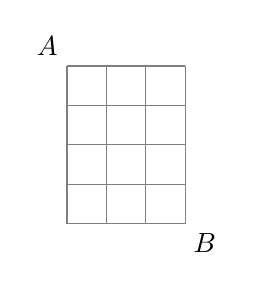
\begin{tikzpicture}
            \draw[step=0.5cm,color=gray] (0,0) grid (1.5,2);
            \node at (-.25,2.25) {$A$};
            \node at (1.75,-.25) {$B$};
          \end{tikzpicture}
        \end{center}

      \item Now we have a much larger grid. This would be very difficult to
        count the paths by hand. Instead, let's try to come up with a recursive
        solution. Let's have the number of paths from $A$ to $B$ be $P$, the
        number of paths from $A$ to $B_1$ be $P_1$, and the number of paths
        from $A$ to $B_2$ be $P_2$. Now give a formula for $P$ in terms of
        $P_1$ and $P_2$

        \begin{center}
          \scalebox{0.75}{
          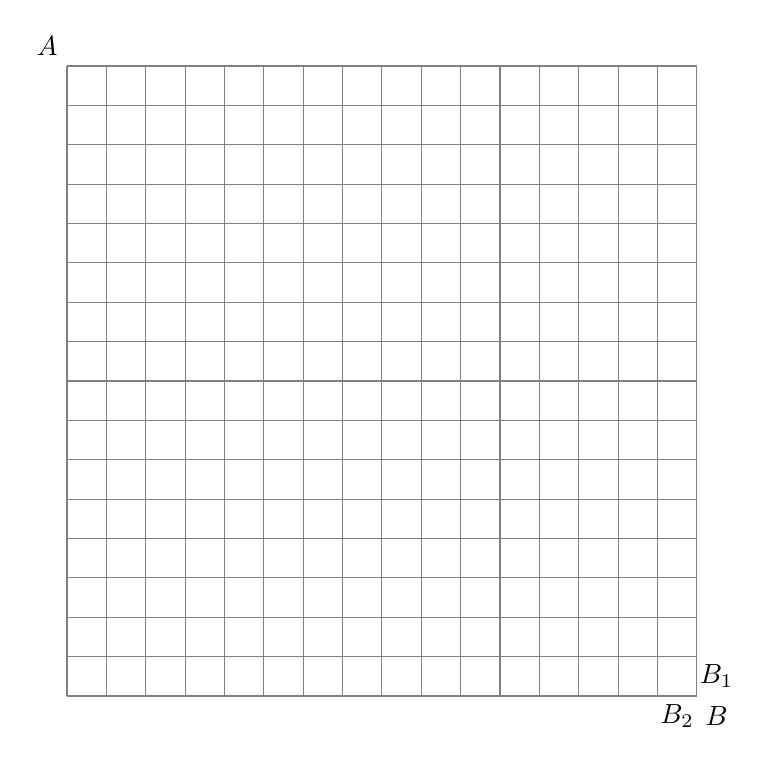
\begin{tikzpicture}
            \draw[step=0.5cm,color=gray] (0,0) grid (8,8);
            \node at (-.25,8.25) {$A$};
            \node at (8.25,.25) {$B_1$};
            \node at (7.75,-.25) {$B_2$};
            \node at (8.25,-.25) {$B$};
          \end{tikzpicture}
          }
        \end{center}

        \begin{align*}
          P=
        \end{align*}

      \item Now given a grid of $r$ rows and $c$ columns, give a recursive
        formula for the number of paths from $A$ to $B$

    \end{enumerate}

%%%%%%%%%%%%%
  \newpage %%%%%%%%%%%%%%%%%%%%%%%%%%%%%%%%%%%%%%%%%%%%%%%%%%%%%%%%%%%%%%%%%%%%
%%%%%%%%%%%%%

  \item (\textbf{Extra Credit})

    \context{I want to answer a simple question from class.
    If I roll n dice, how many possible rolls are there when order doesn't
    matter? We saw in class that if I have 2 dice, the answer is 21.  Let's
    generalize this.

    First Let’s start by calculating the number of ways of rolling 3 dice.}
    \vspace{1em}
    \begin{enumerate}

      \item How many ways are to roll 3 dice where all numbers are distinct?

      \item How many ways are to roll 3 dice two dice have the same value?
        While the order of the dice doesn't matter, the number that rolled
        twice does.

      \item How many ways are to roll 3 dice where all dice are the same?

    \end{enumerate}

    \vspace{1em}
    \context{This way of counting dice seems like a good start, but it seems like it could
    get complicated pretty quickly. We'll need to break it down.

    Notice that in the last part we had 3 cases: all 3 numbers are distinct, 2 numbers are distinct, and only 1 number is distinct.
    So, we should really ask the smaller question:

    ``how many ways are there to roll $n$ dice, where $k$ dice are distinct?''

    We can again break this into 2 questions.}
    \vspace{1em}
    \begin{enumerate}[resume]

      \item How many ways are there to choose the \(k\) values for the \(n\)
        dice?

    \end{enumerate}

%%%%%%%%%%%%%
  \newpage %%%%%%%%%%%%%%%%%%%%%%%%%%%%%%%%%%%%%%%%%%%%%%%%%%%%%%%%%%%%%%%%%%%%
%%%%%%%%%%%%%

    \vspace{1em} \context{
      For the second question we need to how we group the dice of the same value.

      This doesn't seem like a big deal with 3 dice, but let's look at what
      happens when we have 5. If I roll 5 dice and get 2 distinct values (4 and
      1 for example), how many ways can I break that up?

      I could have (1 1 1 1 4), (1 1 1 4 4), (1 1 4 4 4), or (1 4 4 4 4). So there are 4 possible
      ways.

      This gets more complicated with 3 distinct values, so we need a better
      way to solve the problem. I could also write this as I have $m_1$ 1s and
      $m_2$ 4s. I'll call this the multiplicity of a value. So the multiplicity
      of 1 is $m_1$.

      The problem is really asking how many different ways can
      $m_1 + m_2 = 5$. This is good, because it generalizes. If I have 3 distinct
      values, then I'm asking how many ways can $m_1 + m_2 + m_3 = 5$.
    }
  \vspace{1em}
  \begin{enumerate}[resume]

    \item

  \end{enumerate}

\end{enumerate}

\end{document}
